\begin{savequote}[75mm]
Nulla facilisi. In vel sem. Morbi id urna in diam dignissim feugiat. Proin molestie tortor eu velit. Aliquam erat volutpat. Nullam ultrices, diam tempus vulputate egestas, eros pede varius leo.
\qauthor{Quoteauthor Lastname}
\end{savequote}

\chapter{Object representations in lateral visual cortex}
\newthought{Shape is a diagnostic feature} of object identity. Visually similar objects, such as a pear and an apple, can be grouped together by certain shared visual features. On the other hand, different images or views of any one object can look dramatically dissimilar, yet still belong to the same object (REFREF example?). In the first chapter, we established the behavioral ability of rats to perform visual object recognition and quantified their perceptual choices of object similarity. We next turned our attention to the neuronal substrates of these abilities. 

% Neural subtrates of object recog. -- what do we know from primates.
In the primate brain, the ventral visual pathway is thought to transform non-diagnostic, low-level representations of features that may be common to many different objects into high-level representations that are both diagnostic of object identity, or selective for a given object, and robust to variations in particular appearance, or tolerant to identity-preserving transformations. 

Primate visual cortex is arranged hierarchically, with visual inputs from the thalamus first arriving in so-called ``striate'' cortex (also known as area V1), before being processed and forwarded through a successive chain of hierarchically-organized visual areas (area V2 > area V4 > inferotemporal cortex) curving along the ventral surface of the brain. Along each stage of the ventral stream, there is a gradual increase in object selectivity and tolerance, culminating in area IT, at the highest level of the ventral pathway. 

Several key trends have been observed in the response properties of visual neurons as one progresses from ``lower'' to ``higher'' visual areas along this ventral pathway. First, the region of visual space that a given cell responds to (the ``receptive field'') gradually increases as one moves along the ventral pathway, with receptive fields in the highest stages of visual cortex sometimes responding to up to half of the visual field\cite{op2000spatial}. Meanwhile, selectivity for complex object features also increases along the ventral visual pathway, with neurons in later stages of the pathway responding only to very particular configurations of features\cite{Desimone1984, Logothetis1996}.  Critically, as one progresses along the ventral pathway, neurons also exhibit greater tolerance to identity-preserving transformation of the retinal image -- that is, neurons tend to retain their selectivity for particular object features even if those features are, for instance, moved around on the retina, or scaled up or down in size\cite{Ito1995}.These combined features of selectivity and tolerance are in many ways the key computational hallmarks of high-level vision\cite{DiCarlo2007, DiCarlo2012}. 

% Previous rodent studies
\section{Lateral visual cortex exhibits many of the same core properties found in primates}
Anatomical studies have shown that the connectivity of rodent visual cortex observes a similar hierarchical pattern, with thalamic inputs arriving in an analogous striate area V1 in posterior of the brain, and then projecting ventrally to a series of interconnected extrastriate areas\cite{Coogan1993, ETC}. However, while these areas have been characterized anatomically, much less is known about their function.

Since 

% shape selectivity
% natural vs scrambled
% vs. category representations (Vinken)
% tolerance

To determine the extent to which rat lateral visual cortex intrinsically exhibits properties thought to be important for spontaneous, as opposed to learned, object recognition behavior, we recorded from neural populations in awake, naive rats presented with a subset of the same stimuli used for the trained rats (see Chapter 1, Figure\ref{fig:behavior_generalization}) to probe axes of transformation in which object identity is either preserved or gradually morphed to a new identity across changes.


\section{Single neurons exhibit selectivity and tolerance}
One key feature of the primate ventral stream is a gradual increase in shape or object selectivity and a parallel increase in tolerance to identity-preserving transformations. Previous studies have shown that single-units in monkey IT exhibit a trade-of between these properties: neurons that are highly selective are less tolerant to identity-preserving transformations and highly tolerant neurons are not as selective to particular objects\cite{Zoccolan2007}.

To determine whether single neurons exhibited similar characteristics in rat visual areas, we first measured single neuron response profiles in areas V1, LM, and LI. For identity-changing transformations, we tested a subset of the morphs used to probe trained animals’ naive perceptual boundaries (see Figure\ref{fig:behavior_generalization}\textbf{REFREF}), and for identity-preserving transformations, we tested a subset of sizes covering the range of stimulus sizes used to test behavioral generalization to identity-preserving transformations (see Figure\ref{fig:behavior_generalization}\textbf{REFREF}). Since size changes come with large changes in luminance, we also presented a subset of full-screen gray-scale stimuli that were luminance-matched to each size tested (Figure\ref{fig:selectivity_tolerance}\textbf{A}).

\begin{figure}[t!]
    \includegraphics[width=\textwidth]{figures/chapter_4/fig_4-1_single_cell_selectivity_tolerance/single_cell_selectivity_tolerance.pdf}
    \vspace{.1in}
    \caption[Selectivity and tolerance in single neurons]{Selectivity and tolerance in single neurons. \textbf{A.} REFREF.
    \label{fig:selectivity_tolerance}}
\end{figure}

All areas contained a diverse range of object selective and size tolerant cells. For example, even in one V1 FOV, we found cells that exhibited clear size tuning without morph selectivity, morph tuning that was preserved across different sizes, as well as luminance-tuned cells that were also sensitive or insensitive to the different morphs and sizes (Figure\ref{fig:example_blob_responses}). 

Overall, we found that across our object stimuli, cells in LI had the lowest lifetime sparseness, while cells in V1 and LM were similarly high in sparseness (REFREF, stats, Mann-Whitney U Test, multiple comparisons). Since the images varied in morph level and size, the sparseness observedin V1 and LM could reflect a higher selectivity for morph shapes or a lower tolerance for varying sizes. To quantify the amount of object selectivity and tolerance, we calculated a morph selectivity index (MX) and a size tolerance index (ST) for each cell\cite{Zoccolan2007}. We found that relative to V1 and LM, LI cells were both less selective to morphs and more tolerant to size (Figure\ref{fig:selectivity_tolerance}\textbf{E-F}). Notably, this difference was not attributable to overall lower response magnitudes in LI: although we found fewer LI cells selective or responsive to the object stimuli overall, of the cells that were responsive, response magnitudes were comparable across areas (REFREF). 

It is possible that the relatively higher average morph selectivity in V1 and LM cells reflects greater sensitivity to overall luminance values. To characterize the extent to which size or morph tuning simply tracks luminance sensitivity, we calculate the correlation between each cell's size tuning curve and its tuning curve for the size-matched luminance stimuli (Supplemental Figure\ref{fig:supp_X}). While there were indeed cells whose size- or morph-tuning profiles were tightly correlated with broad luminance levels, this was not the case for the majority of cells (V1: 9.8+/-6.8\% of cells with significant correlation between size and luminance tuning across, n=REFREF cells across REFREF imaging sites; LM: 12.6+/-8.2\%, n=REFREF cells across REFREF imaging sites; Li: 12.2+/-9.1\%, n=REFREF cells across REFREF imaging sitse). 

To determine whether rat neurons exhibit a similar trade-off between shape selectivity and transformation tolerance, we calculated the correlation between morph selectivity and size tolerance for simultaneously recorded cells in each imaging site (Figure\ref{fig:selectivity_tolerance}\textbf{G}). 

We found that neurons in rat LM and LI exhibit a strong, negative correlation between morph selectivity and size tolerance (REFREF stats, Pearson’s r=REFREF, p<0.01). Notably, we also saw a negative correlation for V1 imaging sites, as well, but to a weaker degree. To determine whether the strength of this trade-off differed between the three areas, we scrambled each cell’s selectivity index and tolerance index and compared correlation coefficients for those populations that passed the shuffle test (shuffle test, p<0.05 over 5000 iterations, REFREF). We found that correlation coefficients for sites in areas LM and LI were significantly more negative than those in area V1 (REFREF, stats, p<0.05, Mann-Whitney U Test, Bonferroni-corrected for multiple comparisons). 

% A critical property of single neurons in IT is the preservation of rank-ordered object selectivity, that is, relative tuning preference for a set of objects is maintained across changes in identity-preserving transformations such as position or size\cite{Li2009, REFREF}. 

% Arousal?
-Head-fixed, so can monitor arousal with face tracking.
-Larger response magnitudes in high arousal states.
-Overall increase in selectivity (increased shape selectivity and decreased size tolerance)
-signal correlation & noise correlation for High vs. Low arousal
-also, signal correlation & noise correlation as a function of cortical distance. 

% Morphs -- neurometric curves, single-neuron disriminability
-


% Morphs -- population level, arousal effects
\section{Population responses are linearly separable}
Rats accurately classify novel image transformations in the absence of any feedback, suggesting explicit training is not required for generalization behavior (see Figure\ref{fig:behavior_generalization}). However, during behavior, the animal has access to much more than the activity of a single neuron. To determine the extent to which neural populations in rat visual cortex are inherently capable of representations that support discrimination and generalization, we took a population-based approach to compare areas V1, LM, and LI in awake, but untrained rats. Specifically, we trained linear SVMs with neural responses to these same object images to classify the responses as belonging to object A or object B\cite{Hung2005, Li2009, Rust2010, etc}. We then tested the classifiers on each of the two types of generalization tasks performed by the trained rats. 

As done with the behaving animals, prior to the generalization tests, we first measured how well each area could do baseline discrimination between single views of object A and object B. Overall, discrimination accuracy improved with increasingly larger stimulus sizes (Figure\ref{fig:SuppREFREF}). This is consistent with previous single-unit studies of aggregated populations, though here we report performance for simultaneously recorded populations. As expected, we also found better discrimination accuracy for larger neural population sizes (Figure\ref{fig:SuppREFREF}). Only imaging sites that passed this baseline discrimination task were included in further tests of generalization performance (see Methods). 

\begin{figure}[t!]
    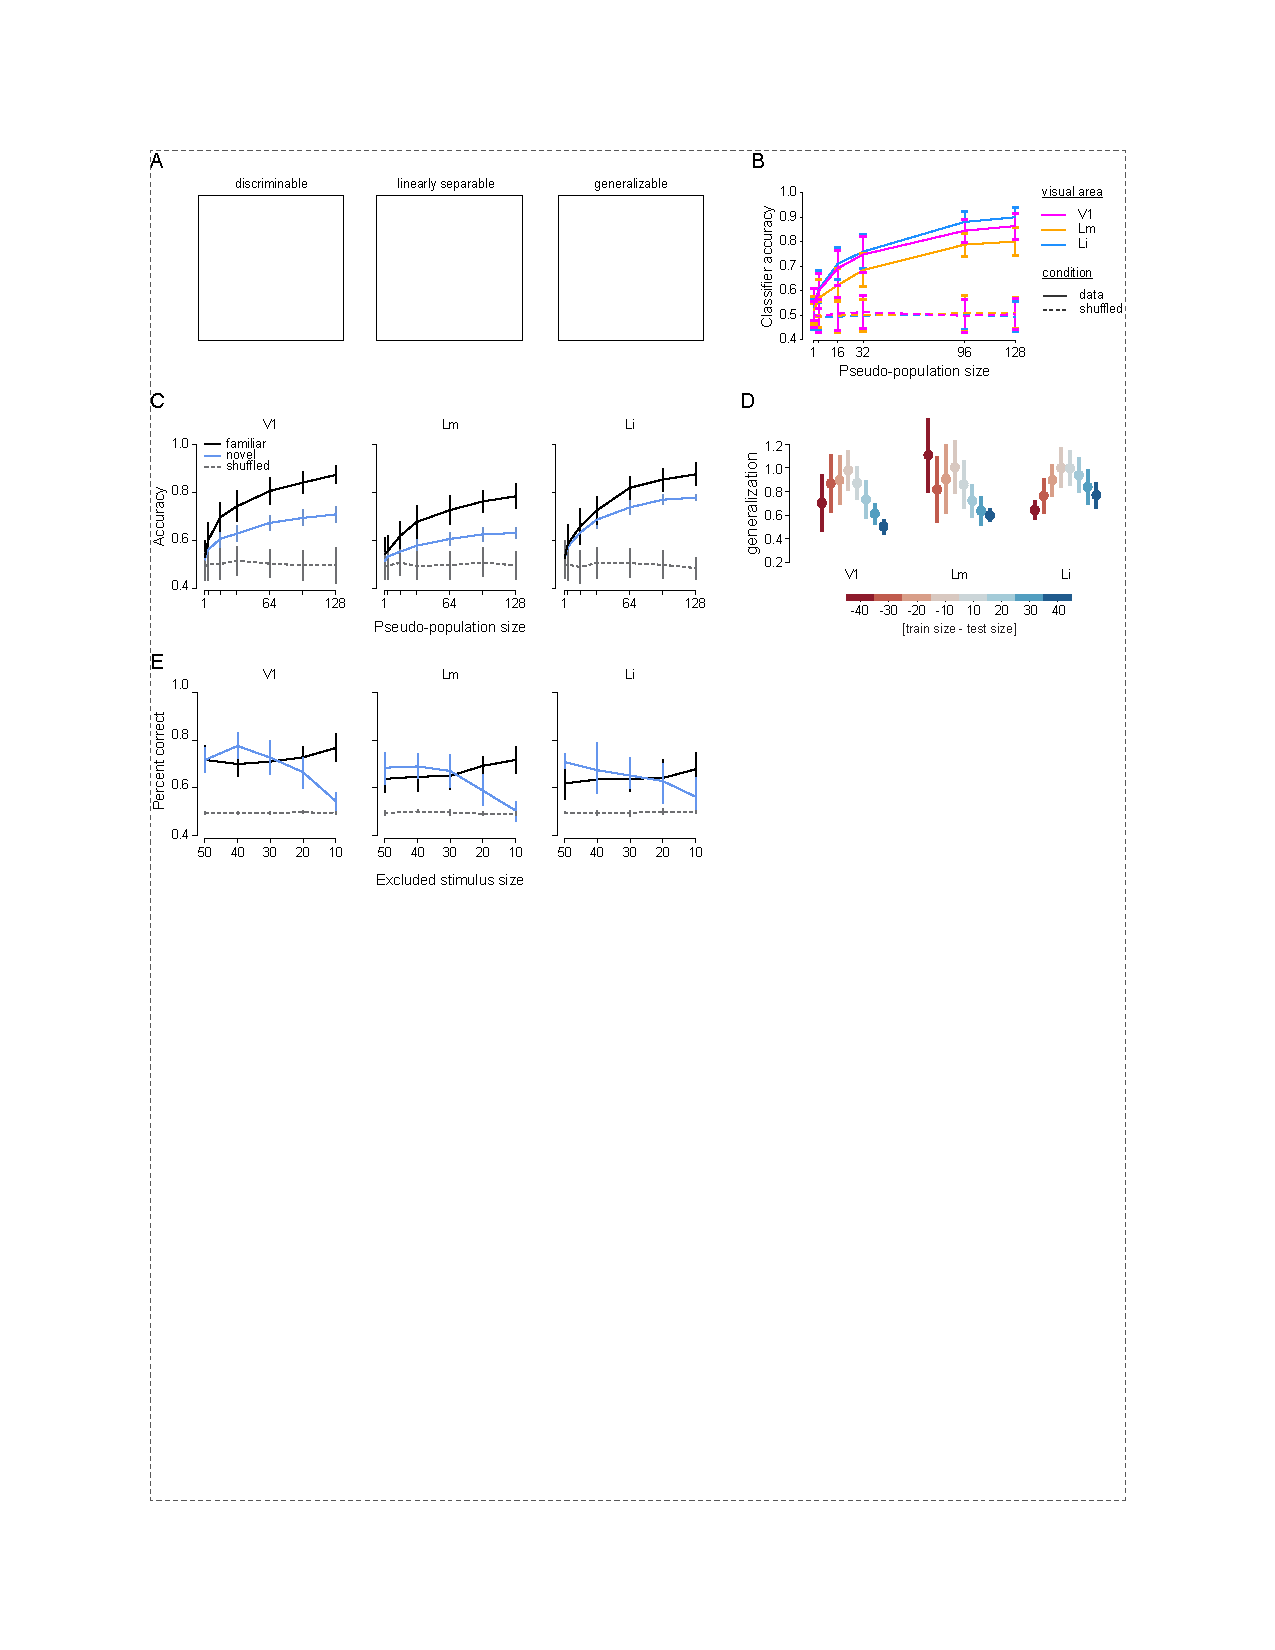
\includegraphics[width=\textwidth]{figures/chapter_4/fig_4-2_neural_generalization/neural_generalization.pdf}
    \vspace{.1in}
    \caption[Selectivity and tolerance in single neurons]{Selectivity and tolerance in single neurons. \textbf{A.} REFREF.
    \label{fig:neural_generalization}}
\end{figure}

We intermediate morphs, which the classifiers have never before seen. Linear SVMs trained on neural data recorded from naive, passive-viewing rats are able to perform this task. 

\begin{figure}[t!]
    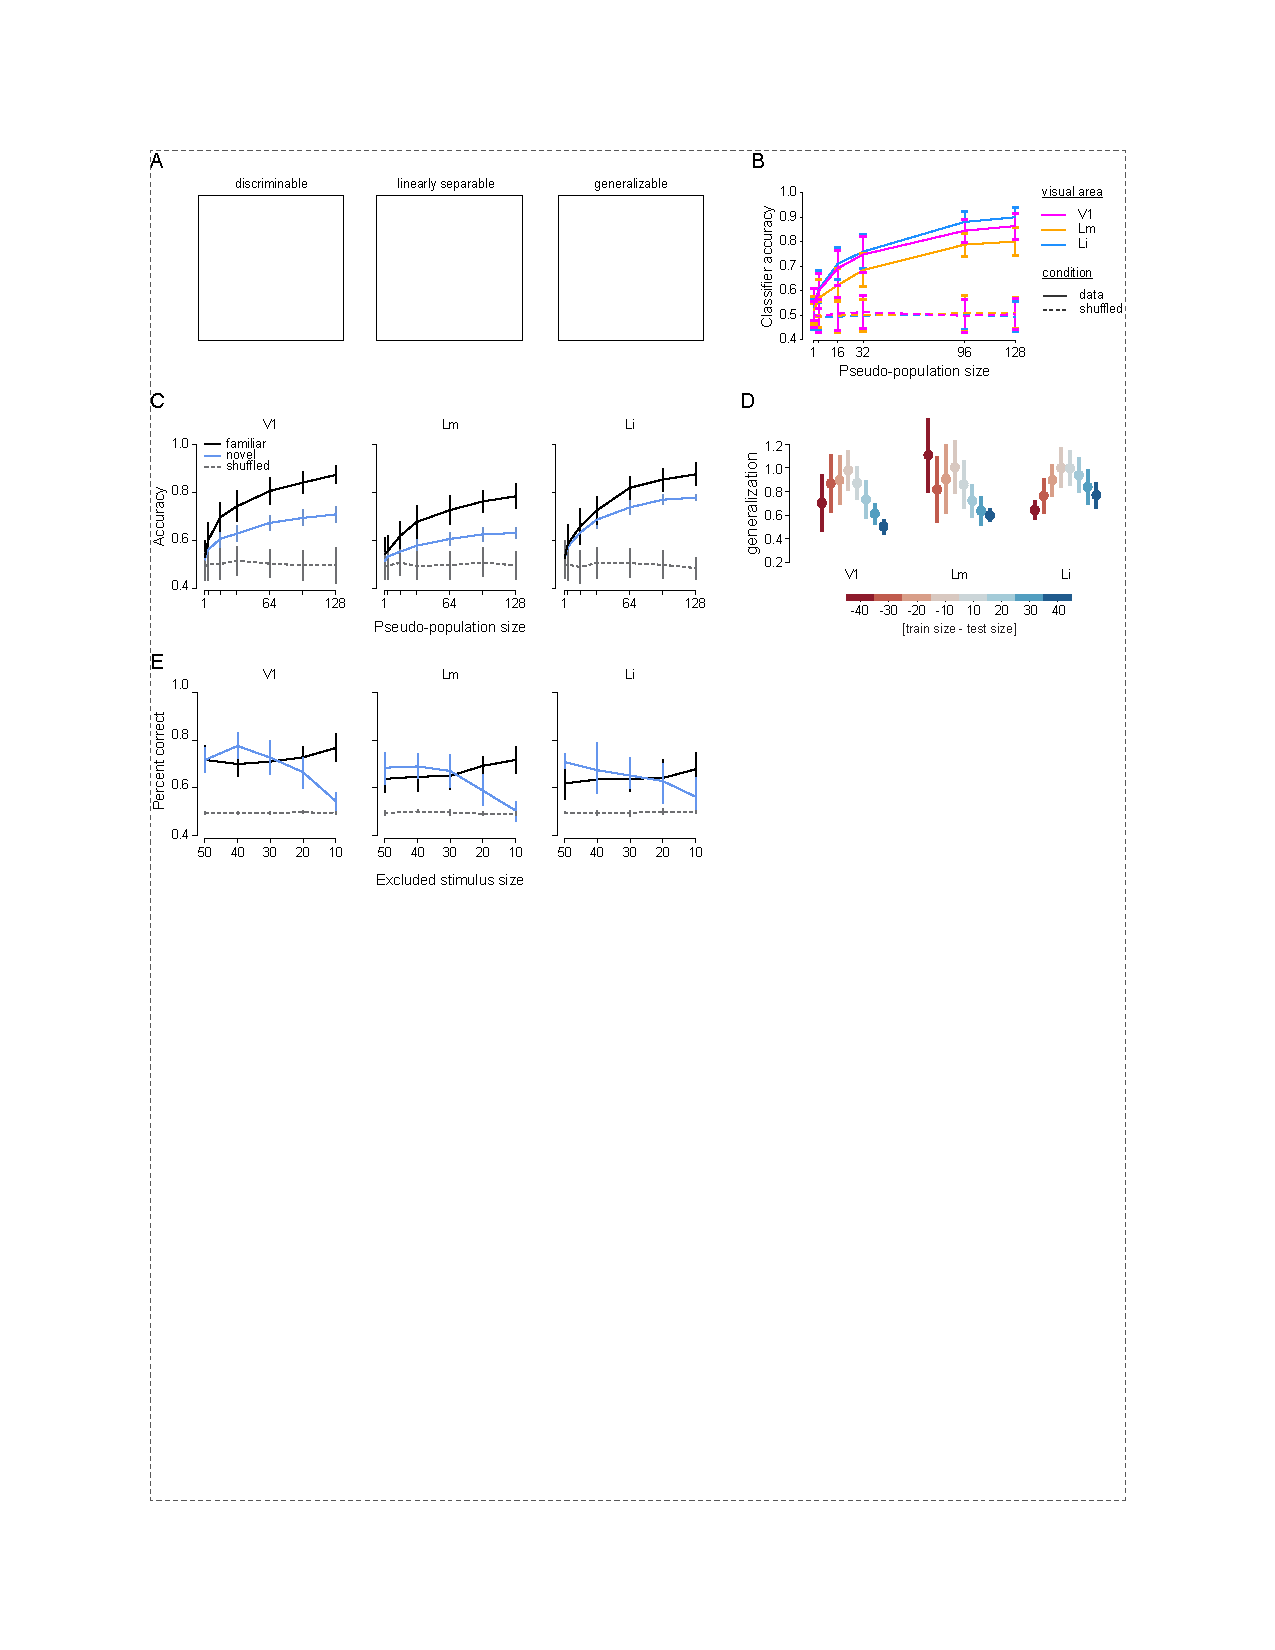
\includegraphics[width=\textwidth]{figures/chapter_4/fig_4-2_neural_generalization/neural_generalization.pdf}
    \vspace{.1in}
    \caption[Selectivity and tolerance in single neurons]{Selectivity and tolerance in single neurons. \textbf{A.} REFREF.
    \label{fig:neural_generalization}}
\end{figure}

To quantify discriminability, we trained linear classifiers (support vector machines) to discriminate the two original objects from the neural activity in each area (Figure\ref{fig:neural_generalization}). The linear-readout scheme is important in that it is a simple, biologically plausible processing step that amounts to a thresholded sum taken over weighted synapses\cite{REFREF}. This classifier approach does not provide a measure for the total information present in the population, but rather estimates the lower bound on the information explicitly accessible to the population to support the visual task. 

Before testing the ability of each population to generalize across identity-preserving transformations, we first tested how well the objects could be discriminated from each other at each of the tested transformations. That is, if a given population failed to discriminate the objects at a given size, failure to generalize to that size would be trivial. For each imaging site, or set of simultaneously recorded cells, in each visual area, we trained linear classifiers to discriminate the two objects at each size, then scored accuracy on trials of the same condition that the classifier had never seen. To avoid trivial generalization due to poor baseline performance, only those populations with average test accuracies greater than accuracies calculated from shuffled object labels were included (p<0.05, REFREF). 

We found that discrimination performance varied as a function of stimulus size, with better accuracy at larger sizes (Figure\ref{fig:REFREF}, stats?). This size dependence was present in all visual areas, and notably, overall performance was comparable across areas, as well. Specifically, average test scores were similar for populations in V1, LM, and LI, with mean scores in V1 and LM being slightly higher, but not significantly different, than LI (mean accuracy +/- std: V1:0.73 +/- 0.08, n=9 sites; Lm: 0.68 +/- 0.04, n=5 sites; Li: -0.64 +/- 0.09, n=4 sites; Mann-Whitney U test, p>0.05 corrected for multiple comparisons).

% Linear separability.
Explain it.
Similar classifier performance as a function of population size. 

% Arousal
Increased shape selectivity could result in better linear separability, but decreased size tolerance could result in worse linear separability. 


% Generalizations.
Size generalization. 
Asymmetric train/test difference



